% Showcase Präsentation mit SimSchoolDark Theme
\documentclass{beamer}

% Theme laden
\usetheme{SimSchoolDark}

% Für Python Code Highlighting
\usepackage{listings}
\usepackage{xcolor}

% Python Code Style
\lstset{
	language=Python,
	basicstyle=\ttfamily\small,
	keywordstyle=\color{simschooldarkest}\bfseries,
	stringstyle=\color{simschoolmedium},
	commentstyle=\color{simschoollight}\itshape,
	numberstyle=\tiny\color{simschoollight},
	numbers=left,
	breaklines=true,
	frame=single,
	rulecolor=\color{simschoolmedium},
	backgroundcolor=\color{simschoolbg!50},
	showstringspaces=false,
	tabsize=4
}

% Präsentationsinfos
\title{ARM-Embedded-Path}
\subtitle{CMSIS-Basics}
\author{Pavel Pys}
\date{\today}
%\institute{}
\begin{document}
	\begin{frame}
		\maketitle
	\end{frame}
	\begin{frame}{Overview}
		\tableofcontents
	\end{frame}
\section{Introduction}
\begin{frame}{Introduction}
	{What is the target of this journey?}
	In these slides, I want to document my learning progress in handling ARM microcontrollers, in my case from the company ST-Microelectronics. Ultimately, this slide set should become a reference work. - Hanover 21.10.2025
\end{frame}
\begin{frame}{Introduction}
	{What is the ARM architecture?}
	\begin{itemize}
		\item A microprocessor architecture developed by the British computer company Acorn in 1983. Initially, ARM stood for Acorn RISC Machine, and was later changed to Advanced RISC Machines.
		\item The company does not manufacture the chips itself, but instead grants different licenses to semiconductor development companies, which then manufacture based on this architecture.
	\end{itemize}
\end{frame}
\begin{frame}{Introduction}
	{What is the ARM architecture?}
	Today, many renowned chip manufacturers build their chips on the ARM architecture.\\
	\textbf{Notable manufacturers:}
	\begin{itemize}
		\item Apple
		\item Qualcomm Inc.
		\item Samsung Electronics
		\item Huawei Technologies Co. Ltd.
		\item ST-Microelectronics
		\item ...
	\end{itemize}
\end{frame}
\begin{frame}{Introduction}
	{Market share of ARM chips}
	The market share of ARM-based chips is very large, but depends on the system. In mobile phones, it was already about 98\% in 2005 (at least one ARM processor). \\
	\vspace{0.2cm}
	In data and server centers, ARM is currently growing rapidly, though its goal of reaching 50\% market share by the end of 2025 is considered ambitious by some analysts.
\end{frame}
\begin{frame}{Introduction}
	{What are the advantages of ARM?}
	The ARM architecture offers several advantages:
	\begin{itemize}
		\item ARM uses the RISC principle.
		\item ARM cores are small and can be easily combined.
		\item Low costs and licensing flexibility.
		\item Large ecosystem.
		\item High performance per watt (efficiency).
		\item Good security features.
		\item Wide range of applications.
	\end{itemize}
\end{frame} 
\section{ARM-Architecture}
\begin{frame}{ARM}
	{What is a Microcontroller Architecture?}
	A microcontroller architecture describes the internal structure and functionality of a microcontroller – meaning how the individual components on the chip are interconnected and how they work together.\\
	\vspace{0.2cm}
	The architecture consists of: CPU, memory, bus system, peripherals, clock source, and power supply as well as reset logic.
\end{frame}
\begin{frame}{ARM}
	{What is a Microcontroller Architecture?}
	In summary: A microcontroller architecture is the blueprint of how CPU, memory, peripherals, buses, and clock sources work together on a single chip to execute tasks efficiently.
\end{frame}
\begin{frame}{ARM}
	{RISC vs CISC}
	\begin{figure}
		\centering
		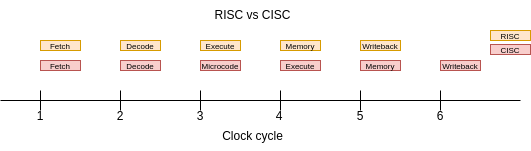
\includegraphics[width=\linewidth]{RISC_CISC_Pipe.png}
	\end{figure}
	The graphic shows the pipelines of RISC and CISC. RISC processes instructions in parallel (one new instruction per clock cycle), while CISC processes longer and more complex instructions sequentially.
\end{frame}
\begin{frame}{ARM}
	{Architecture Structure}
	Register-based design (e.g., 16-32 registers) with a pipeline architecture for parallel instruction execution.\\
	\vspace{0.2cm}
	Harvard or Von Neumann structure depending on the type.\\
	\vspace{0.2cm}
	Components:
	\begin{itemize}
		\item ALU (Arithmetic Logic Unit)
		\item Register set (R0-R15)
		\item Program Counter, Stack Pointer
		\item Interrupt Controller
		\item Bus interfaces (AHB, APB...)
	\end{itemize}
\end{frame}
\begin{frame}{ARM}
	{Architecture Structure}
	Cortex-M microcontrollers typically implement a modified Harvard architecture, where instruction and data buses are separate internally, but share a unified memory space.
\end{frame}
\begin{frame}{ARM}
	{ARM - Cortex M Block-Diagram}
	\begin{figure}
		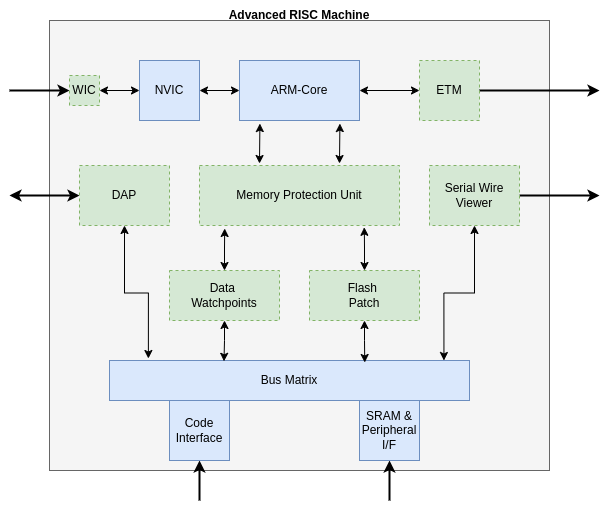
\includegraphics[width=.8\linewidth]{ARM_Block_Diagram.png}
	\end{figure}
\end{frame}
\begin{frame}{ARM}
	{WIC - Wake-up Interrupt Controller}
	In deep sleep (core clock and NVIC logic powered down), the WIC acts as a shadow interrupt latch, allowing selected IRQs to wake the system.\\
	\vspace{0.2cm}
	Control of WIC behavior through:
	\begin{itemize}
		\item NVIC->ISER (enable/disable interrupts)
		\item NVIC priorities and BASEPRI/PRIMASK (only unmasked and sufficiently prioritized IRQs can wake the system)
		\item Sleep depth via SCB->SCR.SLEEPDEEP (Deep Sleep vs. normal Sleep)
		\item WFI/WFE (how you enter sleep)
		\item Peripheral wake sources (EXTI edge, RTC alarm, USART-RX, I²C address match, etc.)
	\end{itemize}
	NVIC is tightly coupled to the Cortex-M core through the System Control Block (SCB), forming the Exception Model
\end{frame}
\begin{frame}{ARM}
	{NVIC - Nested Vector Interrupt Controller}
	The Nested Vector Interrupt Controller (NVIC) is the hardware block in the ARM Cortex-M core that:
	\begin{itemize}
		\item Accepts, prioritizes, nests, and forwards interrupts (IRQs) to the CPU,
		\item Can mask, enable, set/clear pending interrupts,
		\item Integrates exception handling (Reset, NMI, HardFault, SysTick, etc.) using the same mechanisms.
	\end{itemize}
	It is directly integrated into the core, not in the periphery, and coupled with the System Control Block (SCB).
\end{frame}
\begin{frame}{ARM}
	{ARM Core}
	The ARM core is the actual processing core (CPU core) in the microcontroller - meaning the logical unit that executes code, performs arithmetic operations, processes interrupts, and communicates with memory and peripherals via buses.\\
	\vspace{0.2cm}
	In this case (STM32F103), this is an ARM Cortex-M3, based on the ARMv7-M architecture.\\
	This means:
	\begin{itemize}
		\item 32-bit RISC processor
		\item Harvard architecture (separate buses for code and data)
		\item Pipeline design
		\item Thumb-2 instruction set (compact mix of 16- and 32-bit instructions)
	\end{itemize}
\end{frame}
\begin{frame}{ARM}
	{ARM Core: Architectural Features}
	Harvard Architecture:\\
	Separate buses for code (I-Bus) and data (D-Bus) → enables parallel reading of instructions and data\\
	\vspace{0.2cm}
	Thumb-2 Instruction Set:\\
	Mix of 16- and 32-bit instructions → compact code with full functionality\\
	\vspace{0.2cm}
	NVIC Integration:\\
	Interrupt handling directly in the core → no external interrupt controllers needed\\
	\vspace{0.2cm}
	Sleep and Deep Sleep Modes:\\
	Power saving functions via WFI/WFE instructions
\end{frame}
\begin{frame}{ARM}
	{ARM Core: Architectural Features}
	Harvard Concept in Action:
	\begin{itemize}
		\item Instructions are fetched via the I-Bus from Flash memory
		\item Data (variables, peripheral registers) via the D-Bus
		\item System and debug accesses (DMA, DAP, Trace) via the S-Bus
	\end{itemize}
	This allows the Cortex-M3 to simultaneously read an instruction and access data.
\end{frame}
\begin{frame}{ARM}
	{ARM Core: Conclusion}
	The ARM Cortex-M3 core is a 32-bit RISC processor with:
	\begin{itemize}
		\item Efficient pipeline design,
		\item Integrated interrupt controller,
		\item Memory protection (MPU),
		\item Integrated debug/trace architecture (CoreSight),
		\item And ideal for deterministic real-time and embedded applications (e.g., in your STM32F103).
	\end{itemize}
	It is the heart of the microcontroller - all other components (Flash, SRAM, Timer, UART, etc.) are built around it as peripherals.
\end{frame}
\begin{frame}{ARM}
	{DAP - Debug Access Port}
	The DAP (Debug Access Port) is the interface between your debugger (e.g., ST-Link, J-Link) and the internal debug and trace units of your ARM core.\\
	\vspace{0.2cm}
	The DAP acts as the "debug router" between the external world and the CoreSight internals.\\
	\vspace{0.2cm}
	The DAP consists of an AP (Access Port) and DP (Debug Port) interface – e.g. SW-DP for SWD or JTAG-DP for JTAG.
\end{frame}
\begin{frame}{ARM}
	{MPU - Memory Protection Unit}
	The MPU (Memory Protection Unit) is a hardware unit in the ARM core that divides memory into regions and monitors access rights (read/write/execute) for each region.\\
	\vspace{0.2cm}
	It prevents your code from accidentally writing to "forbidden" areas or executing from unauthorized memory.\\
	\vspace{0.2cm}
	It is thus a mini memory protection system, similar to an MMU (Memory Management Unit) in a PC - but simpler and without virtual addresses.
\end{frame}
\end{document}